\chapter{Theory}

\begin{center}
    \textit{This chapter delves into the theoretical foundations of the technologies and methodologies employed in the project. It covers key concepts such as computer vision, image recognition, and the integration of chess analysis tools like \Gls{stockfish}.}    
\end{center}

\section{Literature Review}

With the advancement of technology, various digital applications and solutions have emerged to enhance the experience of playing and analyzing chess. Prominent online platforms such as \textit{chess.com} and \textit{lichess.org} allow players to compete across the globe, offering features such as online matchmaking, tutorials, and game analysis. \\
Additionally, physical chessboards have been modernized through the integration of digital technologies, such as \gls{rfid} tags, which enable the digitization of physical chess games. \cite{quora:shah} \\

Furthermore, advancements in \gls{ai} have led to the development of applications capable of automating tasks such as piece recognition and game digitization. One notable example is \textit{ChessCam}, a web- and mobile-based application designed for quick and efficient live chess digitization. ChessCam allows users to either upload pre-recorded videos of chess games or stream live games using a mobile phone or webcam. The application processes the video input, recognizes the moves, and generates \gls{pgn} files, which can be used for further analysis or archival purposes.

\section{Tools and Technologies}

\textbf{*Brief description of what one might expect to read in the \textit{Tools and Technologies} section*}

\subsection{Version Control}

The use of \gls{git} as a version control system enables collaborative development by allowing multiple developers to work on the same codebase simultaneously. \gls{git} facilitates the maintenance of the code and provides a comprehensive history of all modifications made to the project. These changes are tracked within project containers known as \glspl{repository}, ensuring transparency and accountability throughout the development process. \cite{alphaefficiency:git}

\subsection{Machine Learning}
\label{sec:machine-learning}

\textbf{*Brief description of what one might expect to read in the \textit{Machine Learning} section*}

\subsubsection*{Computer Vision}

% \textbf{*Brief description of what one might expect to read in the \textit{Computer Vision} section*}

As a subfield of \gls{ai}, computer vision focuses on enabling machines to interpret, analyze, and extract meaningful information from visual data, such as digital images and videos. The primary goal of computer vision is to replicate the human ability to perceive and understand visual information, automating tasks that traditionally require human intelligence. \cite{google:vision, microsoft:vision}

\begin{figure}[h!]
    \centering
    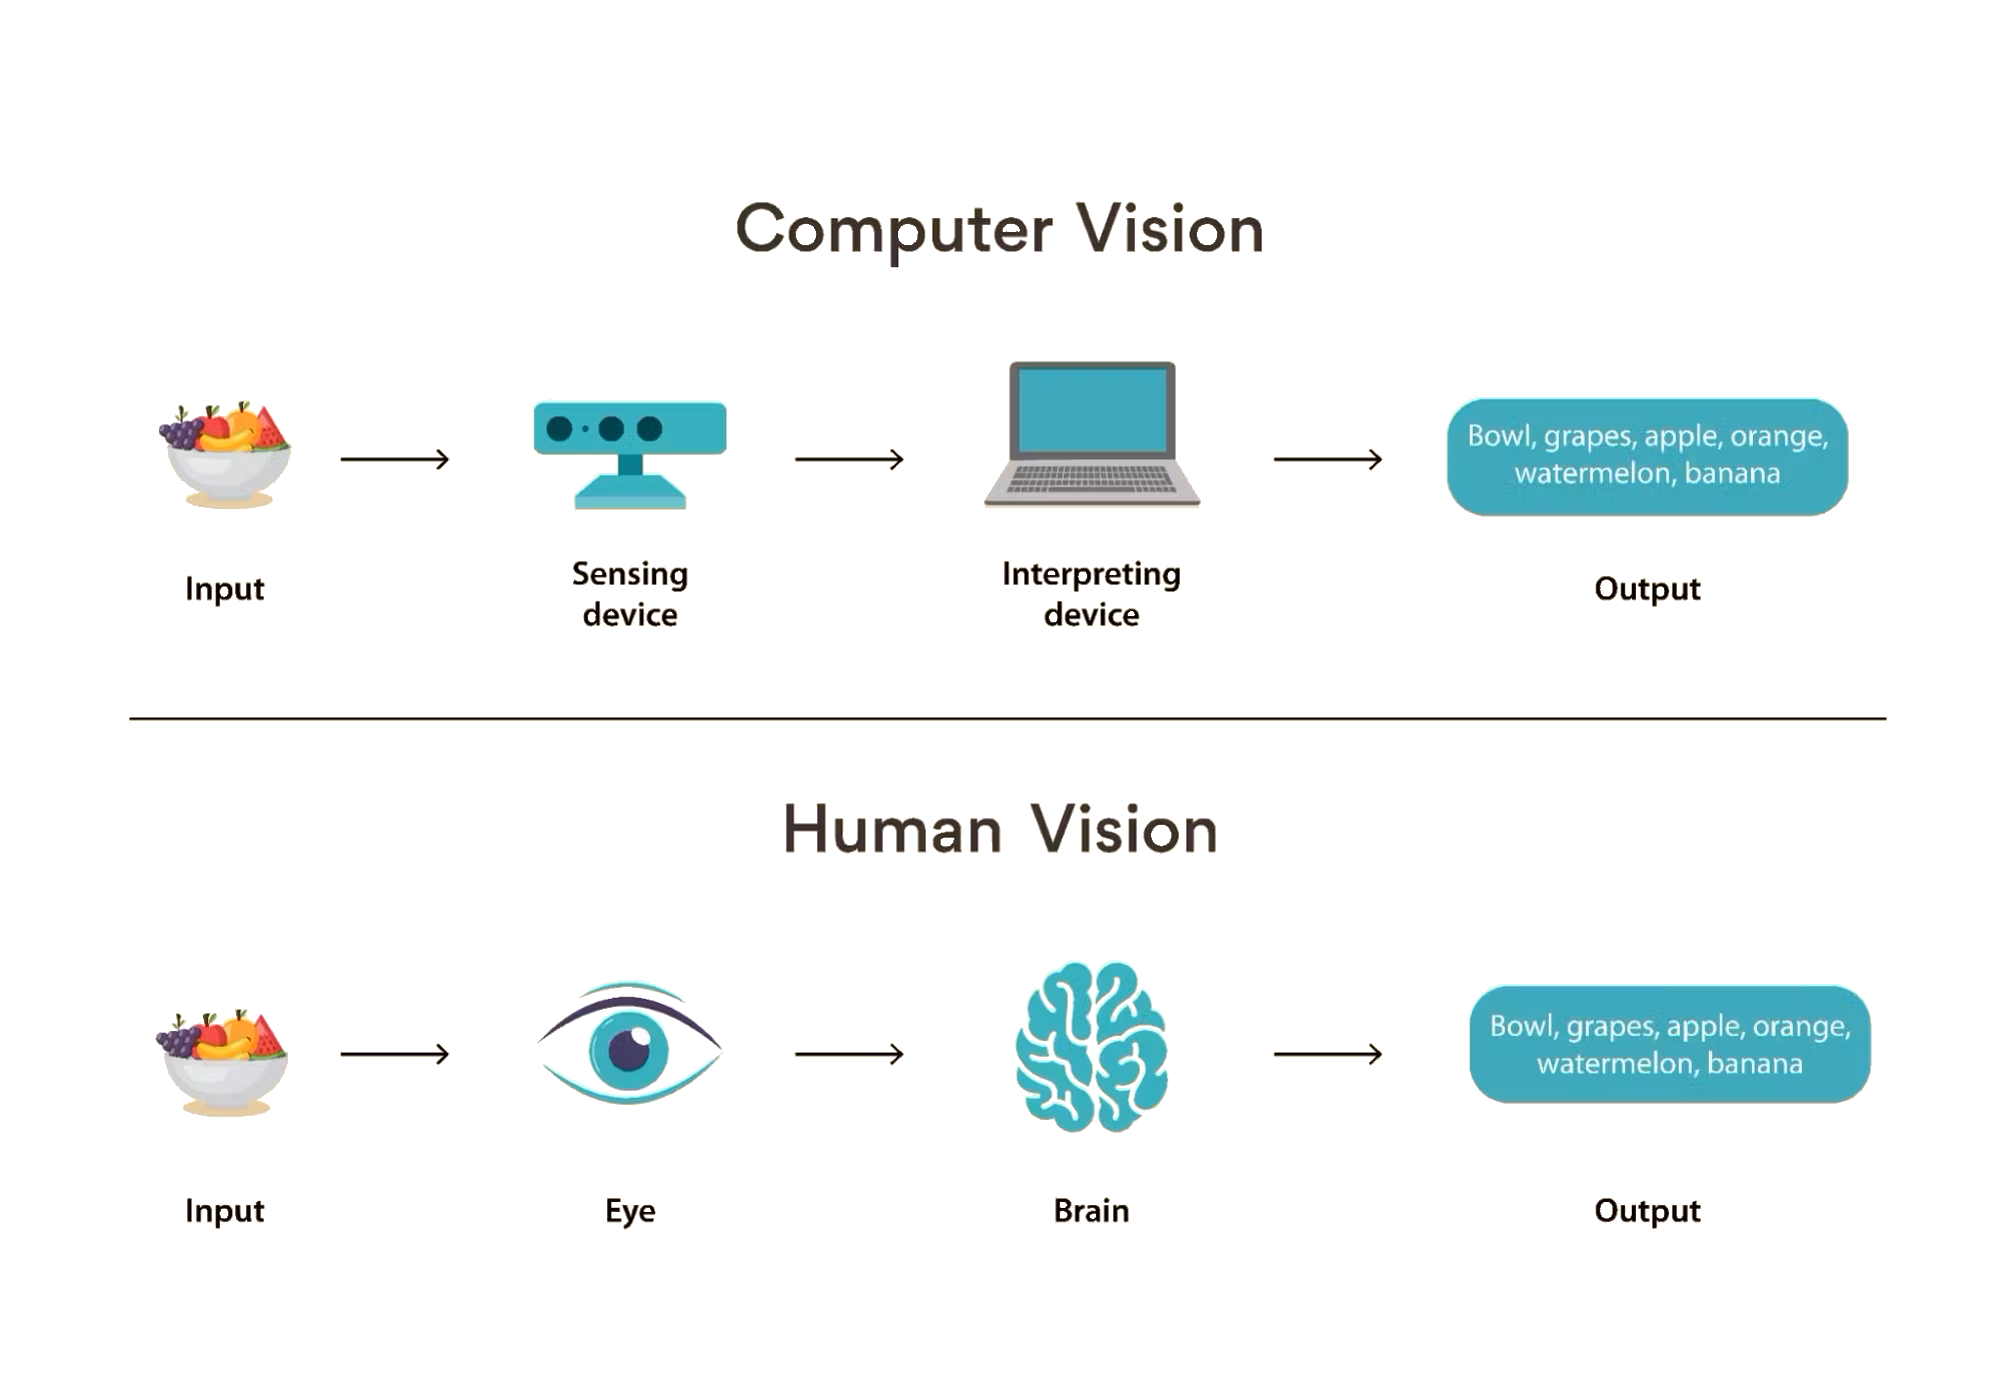
\includegraphics[width=0.75\linewidth]{figures//theory/computer-vision.png}
    \caption{Computer Vision \& Human Vision \cite{turing:computer-vision}}
    \label{fig:computer-vision}
\end{figure}

\subsubsection*{Artificial Neural Network}

Artificial Neural Networks (ANNs) are a cornerstone of modern machine learning, excelling in processing diverse datasets, including images, audio, and text. Different types of neural networks are tailored for specific tasks. For instance, Recurrent Neural Networks (RNNs), particularly Long Short-Term Memory (LSTM) networks, are effective for sequential data like text or time series. In contrast, \glspl{cnn} are specifically designed for image-related tasks, such as image classification, object detection, and segmentation. Their unique architecture, which includes convolutional layers, enables them to automatically and efficiently extract spatial features from visual data. \cite{geeksforgeeks:cnn} \\

\begin{figure}[h!]
    \centering
    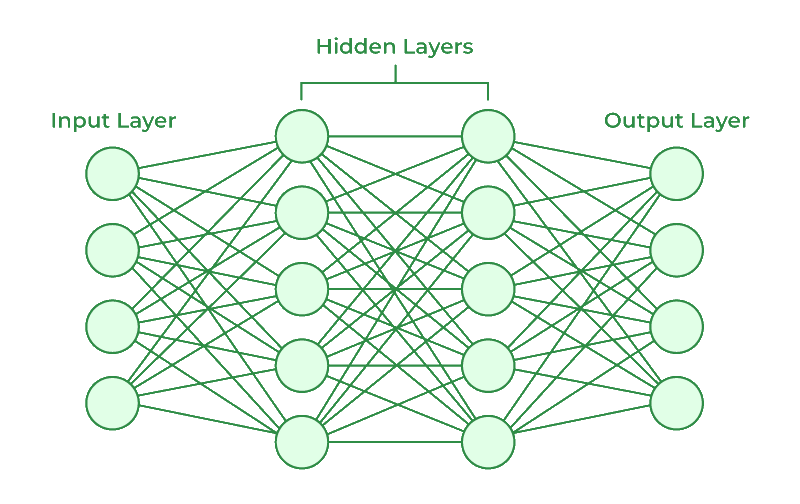
\includegraphics[width=0.75\linewidth]{figures//theory/artificial-neural-network.png}
    \caption{Artificial Neural Networks Architecture \cite{geeksforgeeks:ann}}
    \label{fig:artificial-neural-network}
\end{figure}

The versatility and effectiveness of \glspl{cnn} make them a fundamental tool in computer vision applications, ranging from medical imaging to autonomous vehicles. By leveraging their ability to learn hierarchical representations of visual data, \glspl{cnn} have become a driving force behind many advancements in \gls{ai} and machine learning.

% \gls{cnn} is a specialized deep learning architecture widely used in computer vision tasks. \

\subsubsection*{Supervised Learning}

Supervised machine learning is a fundamental approach for machine learning and \gls{ai}. It involves training a model using labeled data, where each input comes with a corresponding correct output. The process is like a teacher guiding a student—hence the term “supervised” learning. \cite{geeksforgeeks:supervised-learning} \\

The data used in supervised learning is labeled — meaning that it contains examples of both inputs (called features) and correct outputs (labels). The algorithms analyze a large dataset of these training pairs to infer what a desired output value would be when asked to make a prediction on new data. \cite{google:supervised-learning} \\

For instance, pretend you want to teach a model to identify shapes. You provide a labeled dataset that contains many different examples of shapes and the names of each shape. You let the algorithm try to define what set of characteristics belongs to each shape based on the labeled outputs. You can then test the model by showing it a shape and asking it to guess what shape it is, see figure \ref{fig:supervised-learning}. If the model provides an incorrect answer, you can continue training it and adjusting its parameters with more examples to improve its accuracy and minimize errors. \cite{google:supervised-learning} \\ 

\begin{figure}[h!]
    \centering
    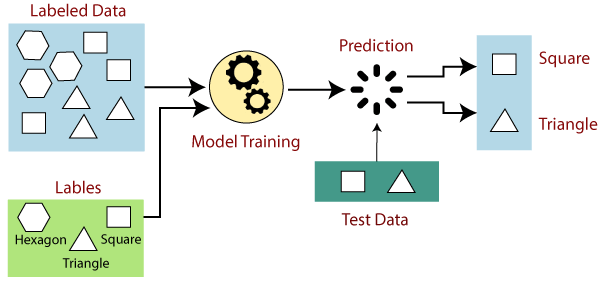
\includegraphics[width=0.75\linewidth]{figures/theory/supervised-learning.png}
    \caption{Supervised Learning Diagram \cite{tpointtech:supervised-learning}}
    \label{fig:supervised-learning}
\end{figure}

Once the model has been trained and tested, you can use it to make predictions on unknown data based on the previous knowledge it has learned. \cite{google:supervised-learning}

\subsubsection*{Classification}

Classification algorithms are used to group data by predicting a categorical label or output variable based on the input data. Classification is used when output variables are categorical, meaning there are two or more classes. \cite{google:supervised-learning} \\

One of the most common examples of classification algorithms in use is the spam filter in your email inbox. Here, a supervised learning model is trained to predict whether an email is spam or not with a dataset that contains labeled examples of both spam and legitimate emails. The algorithm extracts information about each email, including the sender, the subject line, body copy, and more. It then uses these features and corresponding output labels to learn patterns and assign a score that indicates whether an email is real or spam. \cite{google:supervised-learning}

\begin{figure}[h!]
    \centering
    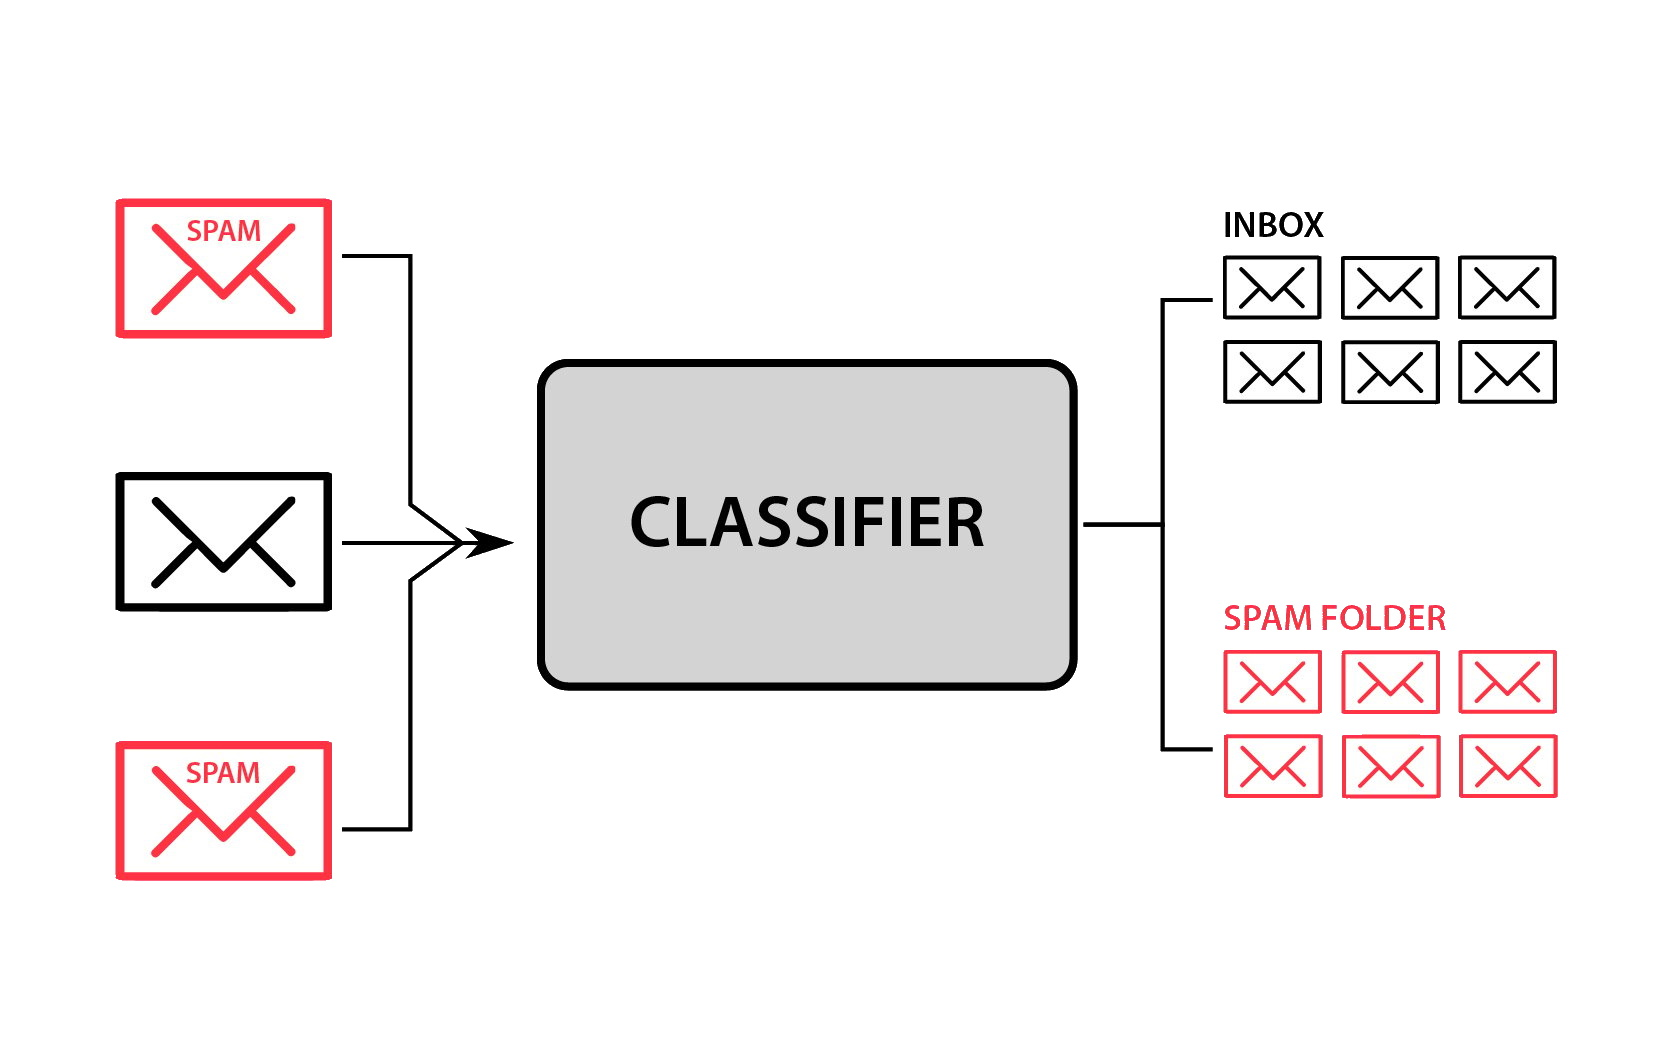
\includegraphics[width=0.75\linewidth]{figures/theory/classification.jpg}
    \caption{Email Classification \cite{analytixlabs:classification}}
    \label{fig:classification}
\end{figure}

\subsection{Web Application}

\textbf{*Brief description of what one might expect to read in the \textit{Web Application} section*}

\subsubsection*{Cross-Platform}

\textbf{*Brief description of what one might expect to read in the \textit{Cross-Platform} section*}

\subsubsection*{Online}

\textbf{*Brief description of what one might expect to read in the \textit{Online} section*}

\section{Design}

\textbf{*Brief description of what one might expect to read in the \textit{Design} section*}

\subsection{Wireframe}

\textbf{*Brief description of what one might expect to read in the \textit{Wireframe} section*}

\subsection{Mockup}

\textbf{*Brief description of what one might expect to read in the \textit{Mockup} section*}

\subsection{UX}

\textbf{*Brief description of what one might expect to read in the \textit{UX} section*}

\subsection{UI}

\textbf{*Brief description of what one might expect to read in the \textit{UI} section*}

\section{Code Quality}

\textbf{*Brief description of what one might expect to read in the \textit{Code Quality} section*}

\subsection{Code Review}

Code review is a critical step in the software development process, where a developer's implementation is examined by one or more peers before it is merged into an upstream branch, such as a feature branch or the main branch. This process provides a second opinion on the solution, helping to identify bugs, logic errors, uncovered edge cases, and other potential issues that may have been overlooked during development. \cite{gitlab:code-review} \\

A well-defined code review process is essential for maintaining high code quality and preventing unstable or faulty code from reaching production. By incorporating code reviews into the team's workflow, software development teams can foster continuous improvement, ensure that all code is reviewed by multiple perspectives, and reduce the risk of introducing defects into the codebase. \cite{gitlab:code-review} \\

Pull requests are a widely used mechanism to facilitate code reviews in modern version control systems. A pull request is a formal proposal to merge a set of changes from one branch into another. It provides a platform for collaborators to review, discuss, and approve changes before they are integrated into the main codebase. Pull requests also display the differences between the source and target branches, making it easier for reviewers to understand the proposed changes and provide constructive feedback. \cite{github:pr}

\subsection{Cohesion and Coupling}

% Coupling refers to the degree of interdependence between software modules. High coupling means that modules are closely connected and changes in one module may affect other modules. Low coupling means that modules are independent, and changes in one module have little impact on other modules. \cite{geeksforgeeks:c&c} \\

% Cohesion refers to the degree to which elements within a module work together to fulfill a single, well-defined purpose. High cohesion means that elements are closely related and focused on a single purpose, while low cohesion means that elements are loosely related and serve multiple purposes. \cite{geeksforgeeks:c&c} \\

% Both coupling and cohesion are important factors in determining the maintainability, scalability, and reliability of a software system. High coupling and low cohesion can make a system difficult to change and test, while low coupling and high cohesion make a system easier to maintain and improve. \cite{geeksforgeeks:c&c} 

Cohesion and coupling are two fundamental concepts in software design that significantly impact the quality and maintainability of a system. \\

% Coupling refers to the degree of interdependence between software modules. In a highly coupled system, modules are tightly connected, meaning that changes in one module may require modifications in others. This can lead to increased complexity and reduced flexibility. On the other hand, low coupling indicates that modules are more independent, with minimal dependencies between them. This promotes modularity, making the system easier to understand, modify, and maintain. \cite{geeksforgeeks:c&c} \\

% Cohesion, in contrast, refers to the degree to which the elements within a module are related and work together to achieve a single, well-defined purpose. High cohesion means that the elements within a module are closely aligned and focused on a specific task, which enhances readability and reusability. Low cohesion, however, implies that the elements within a module are loosely related and may serve multiple purposes, leading to code that is harder to understand and maintain. \cite{geeksforgeeks:c&c} \\

\begin{center}
\textit{"\textbf{Cohesion} refers to the degree to which elements within a module work together to fulfill a single, well-defined purpose. \textbf{High cohesion} means that elements are closely related and focused on a single purpose, while \textbf{low cohesion} means that elements are loosely related and serve multiple purposes."} \cite{geeksforgeeks:c&c} \\
\end{center}

\begin{center}
\textit{"\textbf{Coupling} refers to the degree of interdependence between software modules. \textbf{Tight coupling} means that modules are closely connected and changes in one module may affect other modules. \textbf{Loose coupling} means that modules are independent, and changes in one module have little impact on other modules."} \cite{geeksforgeeks:c&c} \\
\end{center}

\begin{figure}[h!]
    \subfloat[\centering Cohesion]{{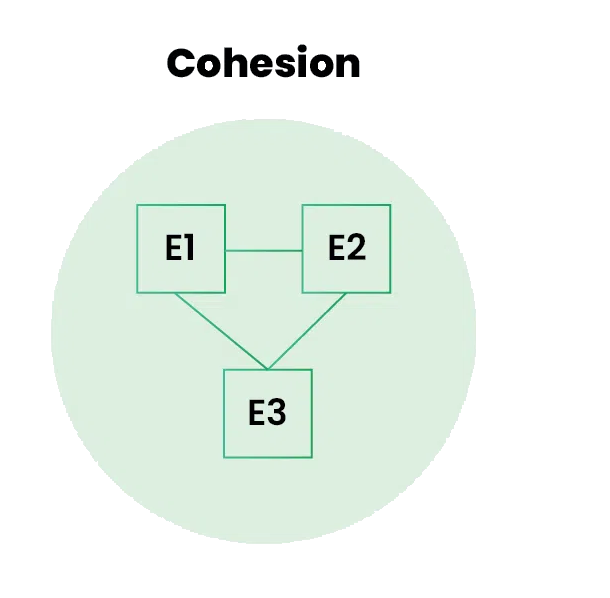
\includegraphics[width=0.5\linewidth]{figures/theory/cohesion.png}}}
    \subfloat[\centering Coupling]{{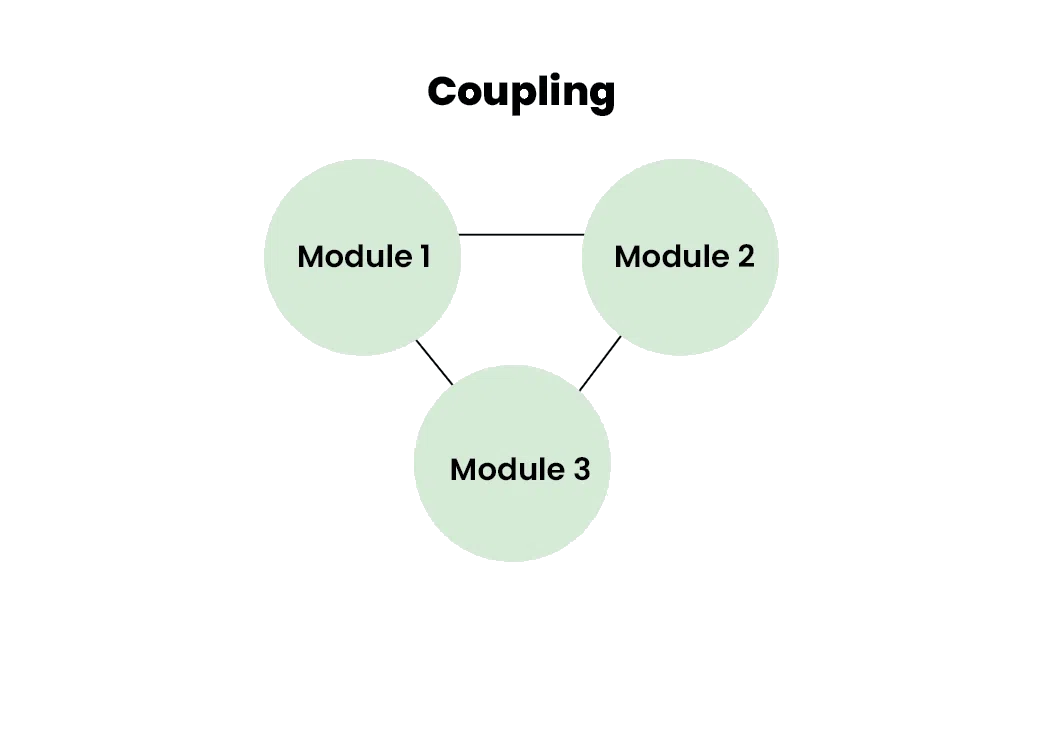
\includegraphics[width=0.5\linewidth]{figures/theory/coupling.png}}}
    
    \caption{Cohesion \& Coupling \cite{geeksforgeeks:c&c}}
    \label{fig:cohesion-coupling}
\end{figure}

Both coupling and cohesion are important factors in determining the maintainability, scalability, and reliability of a software system. Tight coupling and low cohesion often result in systems that are difficult to change, test, and debug. Conversely, loose coupling and high cohesion contribute to systems that are modular, flexible, and easier to improve over time. \cite{geeksforgeeks:c&c}

\subsection{Documentation}

% Documentation is a written piece of text that is often accompanied by a software program. This makes the life of all the members associated with the project easier. It may contain anything from \gls{api} documentation, build notes or just help content. It is a very critical process in software development. It’s primarily an integral part of any computer code development method. \cite{geeksforgeeks:doc}

Documentation is a critical component of software development, consisting of written materials that accompany a software program. It serves as a comprehensive reference for all stakeholders involved in the project, including developers, testers, and end-users. Documentation can take various forms, such as \gls{api} documentation, build instructions, user manuals, or internal design specifications. Its purpose is to provide clarity, facilitate understanding, and ensure the effective use and maintenance of the software. \cite{geeksforgeeks:doc} \\

High-quality documentation is essential for the success of any software project. It simplifies onboarding for new team members, aids in troubleshooting and debugging, and ensures that the software can be maintained and extended over time. Moreover, well-documented code and systems reduce the risk of knowledge loss when team members change or when revisiting older parts of the codebase. \cite{geeksforgeeks:doc} \\

In modern software development, documentation is not merely an afterthought but an integral part of the development process. It should be created and maintained alongside the code, ensuring that it remains accurate, up-to-date, and accessible to all relevant parties.

\subsection{}

\subsection{Testing}

\subsubsection*{Virtual Machine}

\subsubsection*{Unit Testing}

% Unit Testing is a software testing technique in which individual units or components of a software application are tested in isolation. These units are the smallest pieces of code, typically functions or methods, ensuring they perform as expected. \cite{geeksforgeeks:unit-test} \\

% Unit testing helps in identifying bugs early in the development cycle, enhancing code quality, and reducing the cost of fixing issues later. It is an essential part of \gls{tdd}, promoting reliable code. \cite{geeksforgeeks:unit-test}

Unit testing is a fundamental software testing technique in which individual units or components of a software application are tested in isolation. A unit typically refers to the smallest testable part of a program, such as a function, method, or class. The goal of unit testing is to validate that each unit performs as expected under various conditions, ensuring its correctness and reliability. \cite{geeksforgeeks:unit-test} \\

By identifying and addressing bugs early in the development cycle, unit testing significantly enhances code quality and reduces the cost of fixing issues later in the process. It is a core practice in \gls{tdd}, where tests are written before the actual code, promoting a disciplined approach to development and ensuring that the code meets its requirements from the outset. \cite{geeksforgeeks:unit-test} \\

Unit testing also contributes to the maintainability and scalability of a software system. Well-tested units are easier to refactor, extend, and integrate into larger systems, as their behavior is clearly defined and verified. Additionally, unit tests serve as living documentation, providing insights into how individual components are intended to function.

\subsubsection*{Usability Testing}

% Usability Testing in software testing is a type of testing, that is done from an end user’s perspective to determine if the system is easily usable. Usability testing is generally the practice of testing how easy a design is to use on a group of representative users. Several tests are performed on a product before deploying it. You need to collect qualitative and quantitative data and satisfy customers’ needs with the product. A proper final report is made mentioning the changes required in the product (software). \cite{geeksforgeeks:user-test} \\

% Usability testing involves evaluating the functionality of a website, app, or digital product by observing real users as they navigate through it. Typically conducted by researchers, either in-person or remotely, the aim is to identify any areas of confusion or difficulty users encounter while completing tasks. \cite{geeksforgeeks:user-test} \\

% The ultimate goal of usability testing is to uncover pain points in the user experience, revealing opportunities for improvement. By assessing how efficiently users achieve their goals within the product, usability testing helps in enhancing its overall functionality and user satisfaction. \cite{geeksforgeeks:user-test}

Usability testing is a critical aspect of software testing that focuses on evaluating a system from the perspective of an end user. Its primary goal is to determine how easily and effectively users can interact with the system to achieve their objectives. This type of testing involves observing representative users as they navigate through the product, identifying areas of confusion, difficulty, or inefficiency in the user experience. \cite{geeksforgeeks:user-test} \\

During usability testing, both qualitative and quantitative data are collected to assess the product's functionality and user satisfaction. Qualitative data, such as user feedback and observations, provides insights into user behavior and preferences. Quantitative data, such as task completion rates and time-on-task, offers measurable metrics to evaluate performance. Based on the findings, a detailed report is generated, outlining necessary improvements to enhance the product's usability. \cite{geeksforgeeks:user-test} \\

The ultimate goal of usability testing is to identify pain points in the user experience and uncover opportunities for improvement. By understanding how users interact with the product and where they encounter challenges, developers can make informed decisions to refine the design, improve functionality, and increase overall user satisfaction. \cite{geeksforgeeks:user-test}

\subsection{Type Safety}

Type safety is a fundamental concept in software development that ensures the correctness of a codebase by detecting type-related errors during the development process. In dynamically typed languages, such as JavaScript, variables can be assigned values of any type, which often leads to subtle and hard-to-detect bugs. These bugs can be time-consuming to diagnose and resolve, particularly in large or complex codebases. Type safety addresses this issue by enforcing strict type constraints, thereby reducing the likelihood of runtime errors and improving overall code reliability. \cite{dev:type-safety}

\subsubsection*{Key Pillars of Type Safety}

\begin{itemize}
    \item \textbf{Reliability:} Type safety acts as a protective mechanism, preventing runtime errors caused by type mismatches. By ensuring that variables and functions adhere to predefined types, it enhances the stability and reliability of applications. \cite{dev:type-safety}

    \item \textbf{Collaboration:} Explicit type declarations improve code readability and make it easier for developers to understand and work with each other's code. This fosters seamless collaboration, especially in team environments where multiple developers contribute to the same codebase. \cite{dev:type-safety}

    \item \textbf{Efficient Debugging:} Type safety enables early detection of type-related discrepancies, reducing the time and effort required for debugging. By catching errors at compile time (or during development in statically typed languages), it minimizes the risk of runtime failures and simplifies the debugging process. \cite{dev:type-safety}
\end{itemize}

In summary, type safety is a critical aspect of code quality, offering significant benefits in terms of reliability, collaboration, and debugging efficiency. Its implementation, whether through statically typed languages or tools like TypeScript, plays a vital role in modern software development practices. \cite{dev:type-safety}

